%-- \documentclass[11pt,UKenglish, a4paper]{article}
\documentclass[UKenglish]{uiophd}
\usepackage[utf8]{inputenc}
%--fonts--
\usepackage[bitstream-charter]{mathdesign}

%--packages--
%-- tatt ut for uiophd \usepackage[UKenglish]{babel}
\usepackage{csquotes,textcomp,varioref}

%For å kunne gjøre matteting
\usepackage[bitstream-charter]{mathdesign}

%--Sitater i starten av dokumentet--
\usepackage{epigraph}

\usepackage{graphicx}
%--color--
\usepackage[dvipsnames]{xcolor}

%Setter inn pdfer
\usepackage[final]{pdfpages}

%-linespace--
\linespread{1.3}

%-Mer advansert liste--
\usepackage{enumitem}

%--hyperlinks-- include 
\usepackage[colorlinks=false, pdfborder={0 0 0}]{hyperref}

%--fullpage--
%\usepackage{fullpage}

%--Uio-Front-Page--
\usepackage[]{ifimasterforside}

%--bibliography- -sortlocale=nb_No,
\usepackage[backend=biber, sortcites, defernumbers, style=numeric-comp, maxnames=2, natbib=true, backref, sorting=none, url=false]{biblatex}
%fjernet ifra style=authoryear-icomp
\addbibresource[datatype=bibtex]{Remote.bib}


%farger jeg skal ha med
\definecolor{myY}{RGB}{241, 196, 15}
\definecolor{myB}{RGB}{52, 152, 219}
\definecolor{myG}{RGB}{46, 204, 113}
\definecolor{myLy}{RGB}{149, 165, 166}
\definecolor{myR}{rgb}{231, 76, 60}

%--Author and Title--
\author{Simon Lysne Hyenes}
\title{Design for mastery}
\subtitle{Exploring design options for chronic patients}
%--Latex Optimalization--
\tolerance = 5000
\hbadness = \tolerance
\pretolerance = 2000

%--Starter--
\begin{document}

\frontmatter
%\input{titlepage} %--hvis den finnes legges tittelsiden til
\ififorside
\chapter*{Abstract}
\addcontentsline{toc}{chapter}{Abstract}

\chapter*{Acknowledgements}
\addcontentsline{toc}{chapter}{Acknowledgements}
\clearpage
%Insert table of contents and then skip to next page
\tableofcontents
\addcontentsline{toc}{chapter}{Contents}

\clearpage

\listoffigures
\listoftables


\mainmatter
\chapter{Introduction}
	\section{Tom}

\chapter{Theoretical Framework}
	\section{A theory of mastery}
		Younger defines mastery as ``a human response to difficult or stressful circumstances in which competency, control, and dominion have been gained over the experience of stress''\cite[p.76]{Younger1991Theory}. This is not mastery as having mastered a craft or skill but related to one's ability to handle situations. Mastery here relates to a positive outcome from dealing with stressful and difficult situations.
	
		\subsection{Philosophical and Conceptual elements}
			Younger points to stoicism and existentialism as the philosophical and conceptual foundations. Despite their association with futilism they also deal with accepting and confronting reality. as perceived to the fullest of ones abilities. 
			Younger points to four properties of mastery. The first deals with a``sense of control..over a situation that created a sense of vunerability and over ones own life''\cite[p.81]{Younger1991Theory}. The second deals with knowledge of how to deal with and avoid similar events. The third deals with regaining confidence and belief in oneself. The fourth dealing with ``having found alternative sources of satisfaction for what is lost''\cite[p.81]{Younger1991Theory}. Youngers relates mastery also to a higher quality of life. This comes from viewing mastery as not only expressed as an interpersonal relation to oneself but also to others. 

		\subsection{Conceptual Elements}
			\begin{enumerate}[label=\bfseries\arabic*]
			\item \textbf{Certainty}\hfill \\
			Certainty is a state of negotiation ``predominately free of self-doubt'' and somewhat aligned with other involved parties\cite[p.84]{Younger1991Theory}.
			\item \textbf{Change}\hfill \\
			Attempt to reduce stressor by problem-solving, decision-making and action\cite[p.84]{Younger1991Theory}. Younger relates change to our ability to affect fate. As with fate change is the whole-hearted attempt and change may be outside the scope of possibilities.
			\item \textbf{Acceptance}\hfill \\
			Dealing with and coming to terms with the actual circumstances at hand. Reinvest, change or find alternate sources are the main tools for mastering acceptance. Acceptance is the stoic realization of the actual possibilities but also an attempt to move on by reinvesting in new goals or relations. %From Camus and existentialism acceptance allows us to create new meaning and take solace.
			\item \textbf{Growth}\hfill \\
			The last state relates to a positive outcome of the situation through new skills, experience, alternate goals, regained or raised strength. Growth in mastery means a new view of similar events through experience and knowledge. Younger points to this mastery as building a healthier community by a raised ``compassion offer others in similar situations''\cite[p.86]{Younger1991Theory}.
			\end{enumerate}

			These four properties are intertwined, this involves a feedback loop where states may build or destruct other states. Certainty is the conditions and growth the product of mastery. Acceptance and change however may be viewed intertwined elements. Acceptance deals with coming to terms with impossible and change with the possible. Younger points to that change then may lead to ``new knowledge and skills'' and acceptance to ``investment of life energies in new people or new pursuits''\cite[p.87]{Younger1991Theory}. Both of the results allow for change to a state of mastery. 

		\subsection{Timelines and mastery}

			Younger's four properties points to several areas the timeline should strive to support. Mastery depends upon several different stages that cannot be reduced to prescriped actions but depend wholly on the patients intrapersonal mode, experiences and circumstances.

			This support may be considered as either happening during a process of mastery--- or after as a narrative or documentation of a process of mastery. This means supporting different temporal modalities, types of data and levels of use and engagement.   

			The four main properties certainty, change, acceptance and growth all point to different areas the timeline can support. 

			Mastery depends upon certainty and change, this can be supported through examplars of earlier actions. Mastery means constructing ones own story and future reality through acceptance and growth. Acceptance and growth are interpersonal modes that highlight the need to not only focus on past event and actions. Having a focus towards future goals, alternate pursuits outside of the `stressors' may help appectance. Growth may be a state where such as the timeline may have less perceived utility for the patients. It however may still work in the two fashions---as a reminder and a narrative of the process that lead to a state of growth and further as documentation of the altered state that growth lead to. If succesful this awareness further supports the raised compassion toward the community and others. 

			The focus on mastery in contrast with other similar concepts such as autonomy is useful for several reasons. Supporting peoples autonomy means raising or giving people the ability to affect areas that inflict them. Focusing on mastery would mean supporting autonomy--- not as a primary action but as result from self-inflicted change, acceptance and growth.

\chapter{Methodology}

	\section{Participatory Design}


		Participatory design is a research field and design methodology with a special focus on involving users as co-designers in design process. Participatory design has it's roots in the 1970 Scandinavian workplace democracy movement. Participatory design has evolved since the 1970's but it's core value still remains; those affected by a design should have a say in the design process\cite{Simonsen2012Routledge}.

		Greenbaum frames PD within a political perspective where ``people have the right to influence their own lives'' \cite[p.~39]{Hagen2010Social}. This democratic imperative refocuses the design process and emphasises ``genuine participation''\cite[p.~5]{Robertson2006Ethical}. 
		\textit{Genuine participation} of future users and stakeholders expands the possible design space and radically changes the role of designers. 

		Kristen Nygaard pionered the field by working with the Norwegian Iron and Metal Workers Union (NJMF). The goal was to increase both technical and organizational competence among the union workers. Workers feared that their needs where neglected by managements use and implementation of new technology. Early researchers aimed to balance power between management and workers \cite[p.~170]{Kensing1998Participatory}. These efforts has become the Scandinavian approach wih a ``Marxist commitment to democratically empowering workers and fostering democracy in the workplace''\cite[p.~164]{Spinuzzi2005Methodology}. Kensing and Greenbaum point to three theoretical roots: political economy, democracy and feminism\cite[p.~31]{Kensing2013Heritage}. 

		Participatory design has since broadened it's scope and adapted to new issues beyond work/management relations and system development. Today it's used in many different contexts, such as architecture, policy and urban planning\cite[p.~2]{Velden2014RePoliticising}. 

		Kensing and Greenbaum guiding principles reflect the heritage of PD while encompassing current practice:
		\begin{itemize}
		\item{Equalizing power relations}
		\item{Democratic practices}
		\item{Situation based actions}
		\item{Mutual learning}
		\item{Tools and techniques}
		\item{Alternative visions about technology}
		\end{itemize}\cite[p.~33-34]{Kensing2013Heritage}
		These princicples are intertwined and facilitate each other. Bratteteig et. al. points to three core principles: ``Having a say, Mutual learning, Co-realisation''. Participation and democracy are enabled by users having a say through \textit{genuine participation}. Participation and having a say in itself is not enough, participants have to be given legitimate decision power and access to understand the problem area. To work on equal terms there has to be a shared language and socio-cultural understanding\cite[p.152]{Loewgren2004Thoughtful}.  

		Designing the design process is by many considered just as important as the outcome. PD draws upon phenomenological view where every new design practice is unique. Each design practice requires different participants, skills and knowledge domains. The designers role is then as a skilled facilitator whom aims to involve the participants as co-designers.   
		  
		PD is especially appropriate at the earlier stages of the design. To fully utilize co-design with participants means involving users as early as possible.  Allowing users to participate during the ``fuzzy front-end''\cite[p.~6]{Sanders2008CoCreation} gives them access before constraints and visions steer the design process\cite{Loewgren2004Thoughtful}. 

	\subsection{Tools and Techniques}
		PD projects often lead to knowledge about tools and techniques that support these principles. Kensing and Blomberg point to that PD as a community of practice is shaped and defined by the tools and techniques employed: ``strategies that allow for the direct participation of workers in project definition and design specification.''\cite[p.~181]{Kensing1998Participatory}. Research in PD often strive to develop and formulate these strategies for future use. 

		Tools and techniques can be judged by their ability to enable enacting, telling and making. Telling refers to participants ability to having a say. Making activities use creativity to explore future possibilities. Enacting refers to staging and imagining scenarios, allowing participants to enage with future situation and raise mutual understanding\cite[p.149]{Simonsen2012Routledge}. There are several prominent tool and techniques such as future workshop, probes, design games, and storyboards.
		Low-fidelity prototyping is a central technique in PD and used in most projects. Contrary to other design practices prototyping of artifacts may not be specifically aimed at creating better prototypes but as boundary objects for discussion and envisioning futures.

		PD also means taking the needs of the participants seriously. This mean that workshops and other engagements with users need to be engaging and fun. Formal, stiff and strictly procedural techniques are therefore less useful than techniques that engage through playing and doing.\cite[p.153]{Loewgren2004Thoughtful}. Experience and ability to facilitate such work requires both theoretical but also practical knowledge.The ability to converse, lead, guide and raise creativity and engagement essential and Löwgren and Stolterman stress the need to consider practical understanding as a valuable skill\cite[p.152]{Loewgren2004Thoughtful}. 

	\subsection{Why PD in this project}
		The main benefit of using PD is in the belief that the process will lead to not only a better solution but also a learning process of working with teenagers.

		The scope and access means that the project participatory possibilities are limited. This project does not have the possibility to truly utilize participatory design. Despite this PD still offers valuable tools and techniques and an unique research focus. 


		Bratteteig and Stolterman frame the purpose of design as:

		``not just the designed artefact itself, but changes in the range of possibilities for action in the social organization which will use the artefact''\cite[p.~4]{Bratteteig1997Design}.

		Beyond its morals implication this also points to PD ability to engage and work with specific design situations. Its specificity can positively focus and frame loosely defined design problems.  

		The group we are working towards are teenage patients which have a unique situated perspective. The group can be considered domain experts with an understanding of their lifeworld, their wishes, concerns and needs. Cooperation with this group allows for an unique insight and a mutual learning process. The research area involved gaining insight into this domain beyond what I could envision or garner from literature. Technology, culture and society has changed in such ways that envisioning and imagination based techniques fail to capture or reflect these teenagers lifeworlds. 

		Participatory design does not mean that the produced artifacts is the \textit{right} solution or reflect all future use situations. However involving future user raises the possibilities of ``that the product represent the values and meaning of the future users''\cite[p.3]{Velden2014Participatory}. Participatory design on alternative vision also enables escaping trends and the limitations of designers ``technical heritage''\cite{Feng2008Thinking}. 

	\subsection{Design Cycle}
		\begin{figure}
		    \centering
			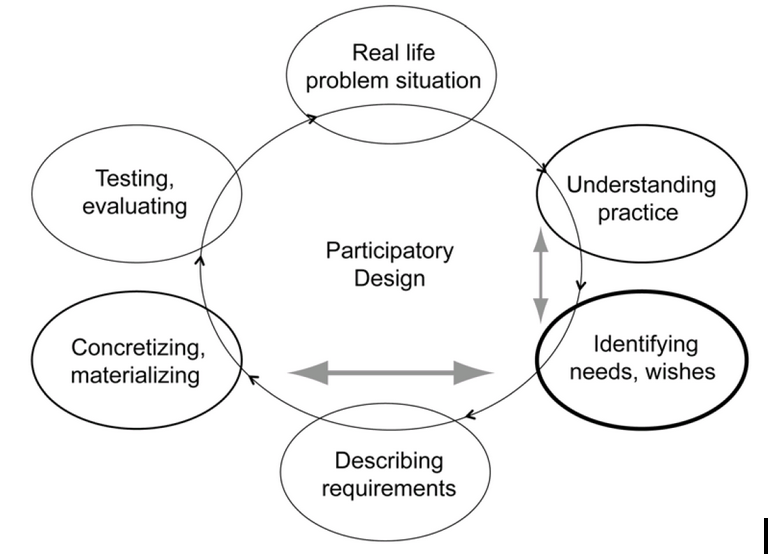
\includegraphics[width=0.5\linewidth]{Images/DesignProcess}
		    \caption{The use-oriented design cycle \cite[p.128]{Bratteteig2013Organising}}
		    \label{The use-oriented design cycle}
		\end{figure}
		There are several design approaches in PD, in this project I am using the use-oriented design cycle. Each stage in the cycle involves different considerations and tools and techniques. The cycle iterates and interplay between identifying needs and concretizing solutions. This reflect Schön's interplay between ``reflection-in-action'' and ``reflection-in-use''\cite[p.~23]{Loewgren2004Thoughtful}.

	\subsection{Ethics}

		From a modern view PD values are related to the ethical stand ``that recognizes the accountability of design to the world it creates and the lives of those who inhabit them''\cite[p.~5]{Simonsen2012Routledge}. As mentioned every design practice is unique. The aim is to allow for \textit{genuine participation}. In doing so meant choosing amongst tools and techniques, focuses and crucially how to frame and present the project's goals. 

		To truly benefit from using PD I tried to involve the users early in the design process. In the beginning this involved focusing the research on the participants lifeworlds and how they related to the proposed problem area. 
		The tools and techniques chosen had to both engage the users but also facilitate mutual learning. This also involves not taking early design decision and instead facilitating the users ability to both explore future vision but also allow for co-realization\cite[p.~10]{Velden2014Participatory}. 

		Considering Dewey’s ``morality in action''\cite[p.~70]{Robertson2006Ethical} every small decisions, soft-coercions, indifference, inclusion/exclusion has a moral and ethical consequence. These choices are ultimately the faciliatators responsibility. Bratteteig et. al discuss \textit{model power}, the symbolic power of the worldviews of the interpreter\cite[p.129]{Bratteteig2013Organising}. The designers role as facilitator and interpretator means that I had to consider my own model-monopoly over the situation. This involved reflecting upon how I related to and understood the user group and their needs. This reflection is especially important considering that the data is inscribed with my interpretations and values. 

		Van der Velden and Mörtberg view PD as a value-centered design approach\cite[p.6]{Velden2014Participatory}. They point to that while PD doesn't ``frontload'' certain values it does enable emerging values through participation and through its methods. In this project certain values are front-loaded by the projects focus while others are implicitly or instrumental such as organizational rules. Van der Velden and Mörtberg describe the ``contact-zone'' as where the design process confronts different interpretations of values and moral. This pluralism means participants and faciliatators may differ in opinion and understanding of certain values\cite[p.~8]{Velden2014Participatory}.

	\section{Outcomes}
		In involving younger patient in the design process and using them as co-designers has several implications. Primarily is the loss of predictability in design solutions. Promoted ideas may contradict or seem foreign. Further divergent solution may come forth within the group. Settling for one coherent vision isn't always possible or practical.

		The solutions will also reflect the lack of involvement of other stakeholders. Their inability to affect what is and isn't within the design space can be both a restriction and a freedom. In this project parents, health professionals and others were neglected to instead focus the limited resources on the patient group. 

	\section{Research through design}

\chapter{Ethics}
	\section{Research with younger adults}
	\section{Research with adolescent patients}
	\section{Reflection}

\chapter{Data Collection}
	\section{NSD}
	\section{User-group}
	\section{Organization of workshop 1 and 2}
	\section{Goals for the data collection}
\chapter{Analysis}

	\section{Thematic Analysis}

		In qualitative studies there are a range of options for analysis and gaining a deeper understanding of the data. Thematic analysis is described by Braun and Clarke as a method for ``identifying, analysing and reporting patterns (themes) within data'' \cite[p.~79]{Braun2006Using}. Thematic analysis is described as a theoretically flexible method, open for different theoretical approaches. This flexibility means that the researchers have to carefully describe their approach and the decisions made before, during and after the analysis. 

	\subsection{Phases of thematic analysis}

		Braune and Clarke's account gives a clear description of the method and divides it into 6 phases. In phase 1 the goal is to ``familiarize yourself with the data''\cite[p.87]{Braun2006Using}. This involves transcribing, reading and starting to form ideas about how to approach the data. 

		In phase 2 the researcher should have an inclination towards what is interesting and present in the dataset. This allows the researcher to code segments which are interesting or pertinent. The idea is to analyse the entire dataset in a similar manner---``giving full and equal attention to each data item''\cite[p.89]{Braun2006Using}. The actual coding process should be done systematically but the tools may range from pen and post-it notes to spreadsheets. Coding should be done liberally including as many themes and codes as feasible, include contextual information and allow for multiple codes on data item\cite[p.~89]{Braun2006Using}.

		In phase 3 the codes should be systematically considered for broader themes. In so each code may be considered and combined with others to form higher themes in the dataset. Braun and Clarke recommend using visual techniques such as mindmaps, tables and card-sorting. The thematic map is then a mindmap including themes, subthemes and relations between the themes. Codes should be within the thematic groups but there may still be codes that aren't grouped.

		In phase 4 the themes are again considered, the ``candidate themes''\cite[p.91]{Braun2006Using} may be combined, split or otherwise rearranged. To do this systematically Braun and Clarke point to Patton's ``internal homogenity and external heterogenity''\cite[p.91]{Braun2006Using}. The themes should be internally logical and in comparison clearly separate. This is done by first considering the codes within each theme to analyse if they are consistent and form a meaningful theme. The second phase is ready when all the candidate themes are ready. The overall themes are then considered in relation to the entire dataset. Here the themes should be considered to what degree they capture and represent the whole. Each theme and the whole set of themes should be considered. The idea is to rework the themes until they can form a thematic map that gives an ``accurate representation''\cite[p.91]{Braun2006Using}. 

		Phase 5 involves naming and further defining themes. This involves a process in which the goal is to ``define and then further refine''\cite[p.92]{Braun2006Using} each theme. The idea is to gain a deeper understanding of what the theme's ``essence''\cite[p.92]{Braun2006Using} is. Here the themes may be considered for sub-themes. 

		Phase 6 is writing and producing a report, the report should be a consistent narrative of the data and analysis ``which convinces the reader of the merit and validity of your analysis''\cite[p.93]{Braun2006Using}. Here extracts and quotes that highlight interesting aspect should be used to ``go beyond description of the data, and make an argument in relation to your research question''\cite[p.93]{Braun2006Using}.

		The phases are all closely related and describe an iterative process of working and reworking the dataset. The first 5 phases all involve moving forwards by reworking previous results. The phases are however useful to focus and promote analytical robustness. It also allows for a systematic way to describe why and how each phase was concluded. There is also a lack of clarity when it comes to finishing recoding codes and reworking themes. The only way to finish is by determining if there is little utility in continued analysis\cite[p.92]{Braun2006Using}.

	\subsection{Workshop 1} 
		For workshop 1 the dataset consisted of the interviews and the drawings. During the first thematic analysis the drawings were only used to consider the codes and inform what they participants were describing. In phase 1 the interviews were transcribed using standard procedures for anonymizing the data. In transcribing the interviews we are refamiliarized with the discussion and also gain insight into the general ideas and topics. It may be done as a purely mechanical exercise. Braun and Clarke however point to the ``interpretive''\cite[p.88]{Braun2006Using} qualitites of transcribing. The act of transcribing involves recording and bringing forwards non-verbal and contextual information. For instance persons entering or leaving the room, multiple conversations, irony, sarcasm, body-language. The goal is to have a rich dataset without the context being ``lost-in-translation''. In transcribing the interviews I attempted to include all such pertinent information. An example was in the drawing exercise pauses and quiet moments where also transcribed. Without it being clear that the participants are drawing the conversation during and after may be nonsensical. For phase 1 the transcription means establishing a bond with the dataset. Several ideas about the dataset became clear but also several problems became apparent. 

		It became clear that the dataset was heavily reliant on the participatory sketching exercise which took a longer portion of time than planned. In the introduction and the beginning of the exercise the data is more pratical than descriptive. The interviews were with groups of respectively 2, 3 and 3 participants. Each group had 20 minutes, within this alloted time there was barely time to gage the participants. Much of the interviews are thin of rich descriptive statements. This would be worse if the interviews was the entire dataset, the sketches however give a deeper insight. 


		After the data was transcribed and reread several times I started phase 2. Here I focused on finding interesting excerpts of opinions, statements and other relevant data. This was coded liberally with several terms and phrases. For each group I first manually annotated and highlighted the interviews using a pen and a marker. With a second copy I did this again using the most useful codes from the first time but also including new codes. The codes were then included in a spreadsheet with the quotations and a remark about the data. 
		From here I started phase 3 which involved sorting through all the codes and trying to find themes that would describe them. The themes should be seen in relation to the research question. The themes are not considered on prevalence alone but on their ability to describe important properties of the dataset in relation to the research questions\cite[]{Braun2006Using}. During this phase a major effort was to allow interal contradictions and include data items that didn't fit within the larger themes. 

		In phase 4 and 5 the themes and their relation to the dataset was considered. It became clear that there was a large number of subthemes that could easily intersect or fit within multiple themes. Separating and sorting the themes was a bit troublesome since so many of the data items had been coded with more than one code. In phase 4 and 5 I worked the following thematic map showing the themes and subthemes as three separate blocks. 

		\begin{figure}
		    \centering
			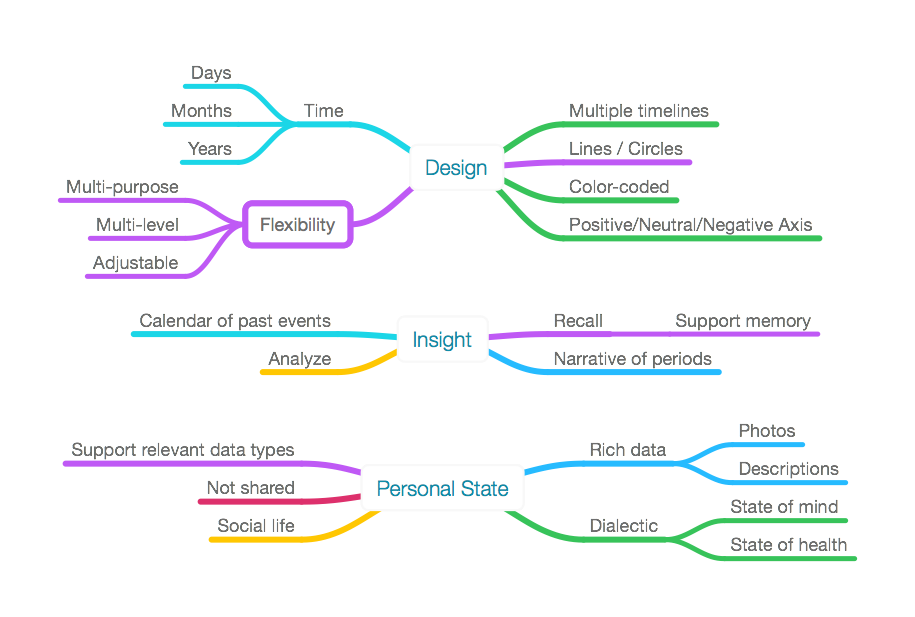
\includegraphics[width=1\linewidth]{Images/ThematicAnalysis}
		    \caption{Workshop 1: Thematic Analysis}
		    \label{fig:1}
		\end{figure}

		The themes describe issues and patterns that were prevalent in the dataset. However determining prevalence in such a short dataset was problematic. This lead to a reduced specificity in the themes. The thematic map has three main themes \textit{design, insight} and \textit{personal state}. Design contains information derived from the sketches and based on statements pertaining to their description of the sketches. Insight is related to the timelines and what the meaning, motivation and outcome such a timeline can provide. Personal state describes the participants main choice for visualization. The participants described their personal state on a holistic level, this qualitative measure was the measure against which other datatypes were considered.

		These three main themes were selected because they could be separated by asking the question of how---design, why---insight and what---personal state. Braun and Clarke point to that themes should be ``internally coherent, consistent and distinctive''\cite[p.96]{Braun2006Using}. The three themes work well in their distinctiveness but less so in internal coherence and consistency. The qualitative codes worked here to describe subthemes, in subthemes which pointed to larger themes. But in doing so there were a range of qualitative choices about groupings which lead to further confusions.

		The findings here are lacking in accuracy and absolutenss due to the number of participants combined with the short-interview time. This was made worse by using participatory sketching where the participant devoted several minutes drawing. Two of the groups were largely consistent and adopted each others ideas while one group were more independent. This was harder to consider when coding since the social dynamics within the participant groups remain unclear. 

	\subsection{Design}
		Design includes subthemes related to the visual and technical properties described by and sketched during the workshop. Several participants described how they would ``click-in'' in the timeline to expand the view from a year to a month, or from a month to a day. This ability to view and scale the timeline was related to working with different types of focuses. From short-term logging to long-term analysis. This was also expressed as a flexibility of the timeline. Such a tool should allow you to compare different types of data and have more than one purpose. For instance one participant wanted to log pain on a 1-10 scale while logging data about both activity levels and activity types. The point being to look at patterns of activities and activity levels that stress and produce a pain reaction.

		Other participants described how documenting was related to their personal needs---``how my body works, if there is a lot of pain, if there is abrasions, if I sleep well, such things that are important for me to maintain control over''. These statements with others were interpreted as a need for a multi-purpose and adjustable timeline. Many of the participants also drew multiple views. Where they had a timeline with datapoints and then another view containing more specific information about that datapoint.

		Lastly the participants used normal conventions such as smily/sad faces for good/bad and red/grey/green for negative, neutral and positive. There were little similarities between the sketches in terms of visual symbols. Several participants included more than one type of data in the timeline for comparison.  
	\subsection{Insight}
		Insight is the themes containing subthemes and data items related to the motivation, purpose and outcome for working with the proposed tool. Several participants mentioned using the timeline as a memory device for recall. Other talked about the analytical possibilities, here the participant describes a use-case without considering the technical and practical concerns: ``you could go in to special days where you see that something special happened\dots What did I do there, that day? Why did it fall? Learn from your mistakes\dots''. The same participant described another use where there is a part of the timeline covering a happy period. Here the participant thought of this as a reminder ``I want something I can look at. Like looking back at this here (points to high-point on sketch)\dots I was glad and my form was good and I know I cant there again that means alot''. 

		One participant described the timeline as a ``calendar of past events''. Several participant mentioned recalling and answering questions related to their health. Here the timeline could be used to log and provide narratives of periods with difficulties or for instance with new medications. More simply one group wanted it to use when ``visiting the doctor and then they ask how have you been the last 6 months and you kind of don't know''. One participant mentioned a journal she had kept to log here stay at the hospital: ``there are many times I have gone and looked at the book at what happened then. A bit to reminisce (neutrally)''. In this context the timeline would be more of a narrative tool than a visualization and it should strive to accurately and truthfully represent the users life-worlds. 
		\subsection{Personal state}
		Personal state is used here to liberally contain themes related to the holistic sense of wellness. The participants described and sketched several different datatypes such as pain, activity and happiness. These datatypes were however always compared back to the overall state of being. Several participants included this as their main timeline. With an vertical axis of postive, neutral and negative personal states. There was an intentional ambiguity that one participant expressed as ``feelings and health (form) are two separate things\dots but of course they interact'' another expressed it as ``I could have written alot here but its in a way, mind and mood''. 

		The participants largely described personal state as a dialetic over time where one day was clearly positive and another negative. The personal state could be summarized as the answers to the question: ``How are you?''. When probed the participants described how each datapoint could contain photos, notes, descriptions, colors to clarify and provide context. Several participants described this qualitative data as neccessary to understand extremes or sudden changes. They also proposed that social activities and friendships could be included as they were integral to their \textit{state of mind}. One group considered sharing the data in the app, but quickly realized that it was to personal. It's proposed purpose and strenght depend upon its ability to be personal. 

		Participants described logging data types relevant to their specific needs. As previously mentioned two participants wanted to log pain, training, activity and abrasions while others mentioned medicines, sleep and mood. Largely they described the two types, simple numerical scales and qualitative data. 

	\subsection{Discussion of the results}
		In workshop 1 there were eight participants that each sketched a timeline. From reviewing the transcription it became clear that the sketching exercise was started without steering and ended rather quickly. This was done because of the time and the participants. Largely the sketches worked to engage and start the discussion. Of the 8 participants 1 sketched a drawing without any meaningful content, the other 7 participants all made original contributions of varying quality and fidelity. Most of the sketches are crude and simple but they describe and show several instering aspects. However due to the very short time period they were made in they should not be considered as prototypes but as objects-of-discussion. 
		During the sketching session the participants contributed with several original ideas and where more open to qualitative data than expected. It is however unclear if they will find logging and using such data as meaningful.

		From visualization literature and research there has been little concentration on mixing qualitative data with automated visualizations. (mer her)

		Based on the result from the workshop it became clear to me that the focus should be towards expressing some aspect of the participants life-world that can provide insight. There should be less emphasis on the transforming the data to visualize meanings or patterns and instead focus on providing long-term and short term narratives. In the analysis it became clear that the participants wanted some focus on their \textit{personal state}. 
		This points to two alternatives, a standard timeline of personal state combined with other data or a timeline customized for insight. 

		The first alternative is a timeline that shows a simplified \textit{personal state} visualized over time, with other qualitative or quantitative data such as images, notes or other annotation illustrated but not shown on the main timeline. This timeline would have different views based on the time perspective--- day, month or year. It could also support several data types such as mood, pain or energy.

		The second alternative is less clear but would entail a customization where each users can create different datatypes they want to log. The datatypes then describe for that users their self-defined progressive \textit{personal state}. For instance two participant mentioned logging pain as especially useful. For them this may be their primary focus, however it could/should be combined with other datatypes such as \textit{personal state} or activity level. 

		Other alternatives that were included in the sketches were calendars, reminders, logging food. At this point such features are less interesting as they are not directly related to the research questions. 

\chapter{Design Proposal}
\chapter{Evaluation of Design and Research Process}
\chapter{Discussion}
\chapter{Conclusion}
\backmatter
%--\subfile{Mastery/MasterySub}
%--\subfile{Time/time}
%\subfile{DataCollection/SemiInterviews/SISub}

%Her skal filen være avsluttet
\clearpage

%Bibligrafien
\printbibliography
\addcontentsline{toc}{chapter}{Bibliography}

%Appendix
\appendix
\chapter{1}
Noe
\chapter{2}
Noe annet
\end{document}